\chapter{矩阵乘优化与性能评估}\label{chap:GEMMOpt}

\section{实验配置}
\begin{table}[htbp]
	\bicaption{实验平台硬件主要参数}{Experimental platform hardware main parameters}
	\label{tab:hardwareplatform}
	\begin{center}
		\begin{tabular}{ | l | p{6cm} | p{6cm} |}
			\hline
			服务器 & ICT NCIC AMD Fiji服务器 & 曙光VEGA服务器 \\ \hline
			GPU & Fiji R9 Nano & 2 Vega10 \\ \hline
			CPU & Intel(R) Xeon(R) CPU E5-2680 v3 @ 2.50GHz & 2 AMD EPYC 7451 24-Core Processor \\ \hline
			内存 & 251GB DDRM & 251GB DDRM \\ \hline
			操作系统 & Ubuntu16.04 & Ubuntu16.04 \\ \hline
			操作系统内核 & rocm-1.7 & rocm-1.7 \\ \hline
			OpenCL C version & OpenCL C 2.0 & OpenCL C 2.0 \\ \hline
			PCIe version & PCIe Gen3 & PCIe Gen3 \\
			\hline
		\end{tabular}
	\end{center}	
\end{table}

本文实验的测试环境包括ICT NCIC AMD FIJI服务器和曙光VEGA服务器。每个计算节点的硬件主要参数如表\ref{tab:hardwareplatform}所示。


\section{矩阵乘性能调优}

\subsection{寄存器分块对v\_mac指令占比的影响}
\begin{figure}[htbp]
	\centering
	%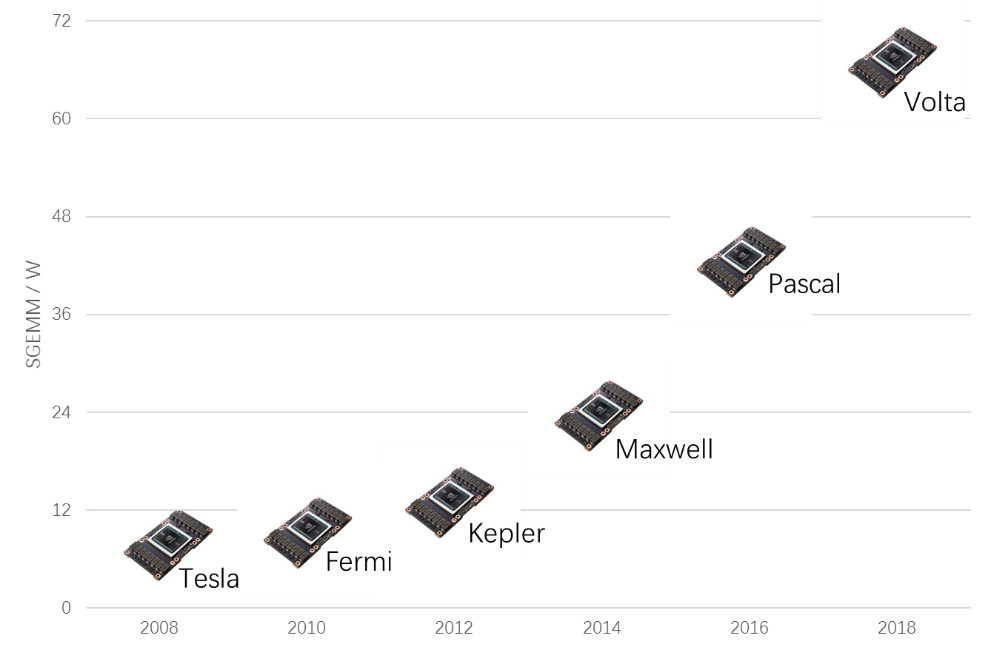
\includegraphics[width=0.40\textwidth]{nvidia_roadmap}
	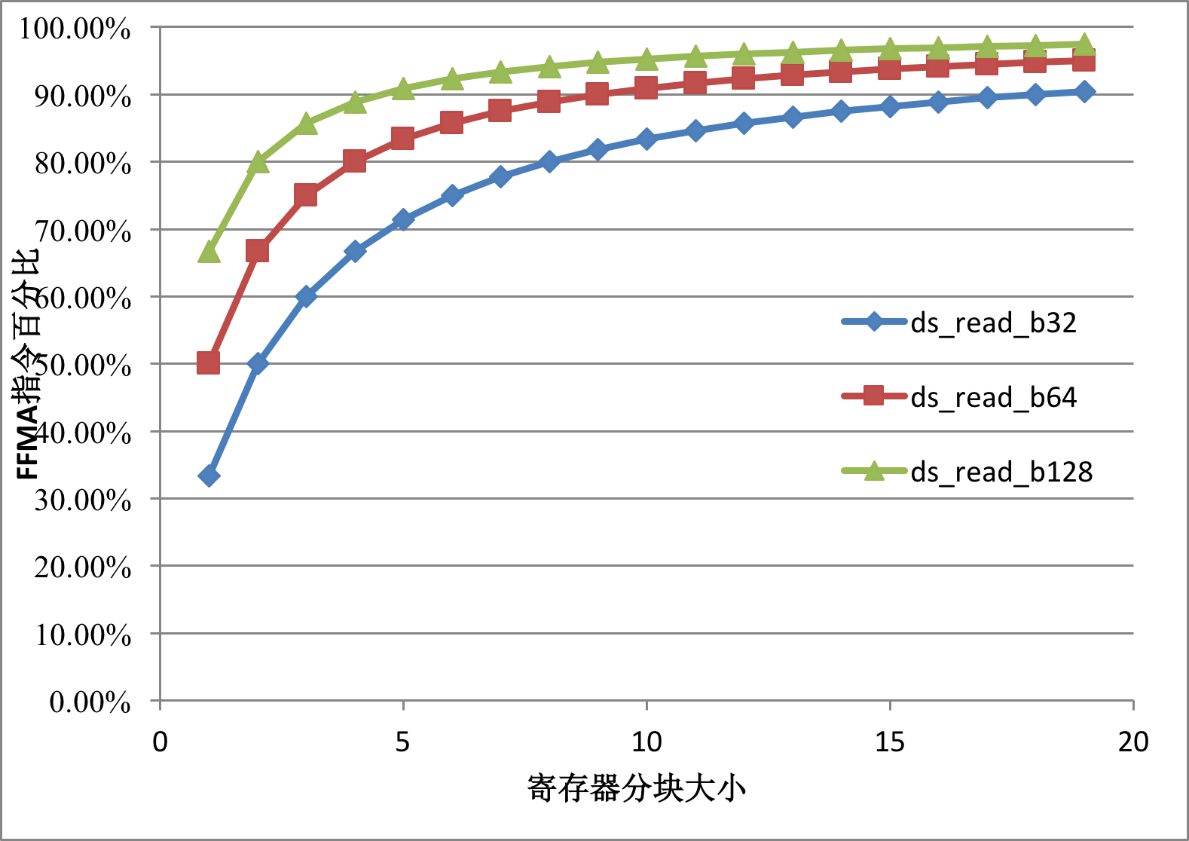
\includegraphics[width=0.50\textwidth]{ffma_percentage}
	\bicaption{v\_mac指令百分比随着寄存器分块大小的变化趋势}{The percentage of v\_mac instruction changes with the size of the register block}
	\label{fig:ffma_percentage}
\end{figure}

从上图中我们可以看出,随着寄存器分块大小增大,v\_mac指令百分比在提高。在寄存器分块大小不变的情况下,ds\_read\_bxx指令的位数宽度越宽,v\_mac指令百分比越高。如果我们采用的寄存器分块大小为6,则FFMA/DS\_READ\_B32=4:1,FFMA/DS\_READ\_B64=8:1,FFMA/DS\_READ\_B128=16:1。FFMA指令的百分比分别为80\%,88.89\%和94.12\%。

增大寄存器分块可以提高v\_mac指令的百分比,在v\_mac和ds\_read混合指令通量不变的情况下,v\_mac指令的百分比越高,v\_mac指令的通量越高。

\subsubsection{使用更宽的数据读指令}
为了实现更好的性能,我们十分有必要将辅助指令的占比减到最小。这里的辅助指令是指非计算指令,尤其是指ds\_read指令。AMD GPU汇编提供了ds\_read\_b32,ds\_read\_b64和ds\_read\_b128指令,分别可从shared memory一次读32bit,64bit和128bit数据。使用更宽的读数据(load)指令可以减少ds\_read指令的数量。

对于AMD Fiji和Vega GPU,每个CU每一个shader cycle的ds\_read指令通量的峰值为32个32-bit。AMD GPU每个CU上每个SIMD有16个LD/ST单元,使用ds\_read\_b64就可以满足通量峰值,所以使用ds\_read\_b128指令不会增加读数据的通量。此时,在ds\_read\_b64和ds\_read\_b128和v\_mac混合指令通量相同的情况下,最好的情况是合理使用ds\_read\_b128指令,使用ds\_read\_b64的通量峰值将是ds\_read\_b32通量峰值的2倍。


\section{汇编层次调优}
我们在实现SGEMM时不会超过预估的SGEMM性能上界。我们对性能上界的评估比较理想化,因为我们主要考虑了影响性能的几个主要因素。除了我们考虑到的几个因素,也有其他因素可能会影响性能。实际的性能上界将介于预估性能上界和实际SGEMM性能之间。

根据A,B矩阵是否转置,我们的SGEMM kernel可分4种情况,NN,NT,TN,TT(N表示不转置,T表示转置)。在我们的分析中,主要考虑了两种类型的指令v\_mac和ds\_read\_bxx。在SGEMM中,还有其他的“辅助”指令对GFLOPS并没有贡献。“辅助”指令包括全局内存地址计算指令,shared memory地址计算指令等。同时,我们也没有考虑barrier指令对性能的影响。任何barrier指令都会降低程序性能。

\subsection{汇编调优的必要性}
使用高级语言(如OpenCL,CUDA)编写GPU程序的好处是开发速度快、易维护,但其对指令的控制能力相对较弱。同时,程序编制人员对编译器的具体行为无法预测。有时,编程人员对OpenCL或CUDA kernel所进行的手工优化可能会被编译器忽略掉。所以,有时候,我们的GPU程序性能会取决于编译器是否友好。

通过编写汇编kernel,编程人员可以直接跳过编译器,面向GPU硬件指令编程。这使得我们有机会进行更细粒度的程序调优。我们可以通过数据预取,寄存器双缓冲,shared memory双缓冲,bank冲突消除,指令重排等手法进行矩阵乘调优。其中OpenCL和汇编都可以使用数据预取,寄存器双缓冲和shared memory双缓冲和bank冲突消除这些手法进行程序优化。但只有通过汇编,我们才能进行细粒度的指令重排。在大量乘加指令之间的合适位置插入访存指令,尽可能用计算掩盖访存延迟。使得矩阵乘主循环中v\_mac指令通量接近v\_mac通量上界。

图\ref{fig:opencl_gemm_1_1}展示了OpenCL实现的矩阵乘不同优化方法的性能比较。

\begin{figure}[htbp]
	\centering
	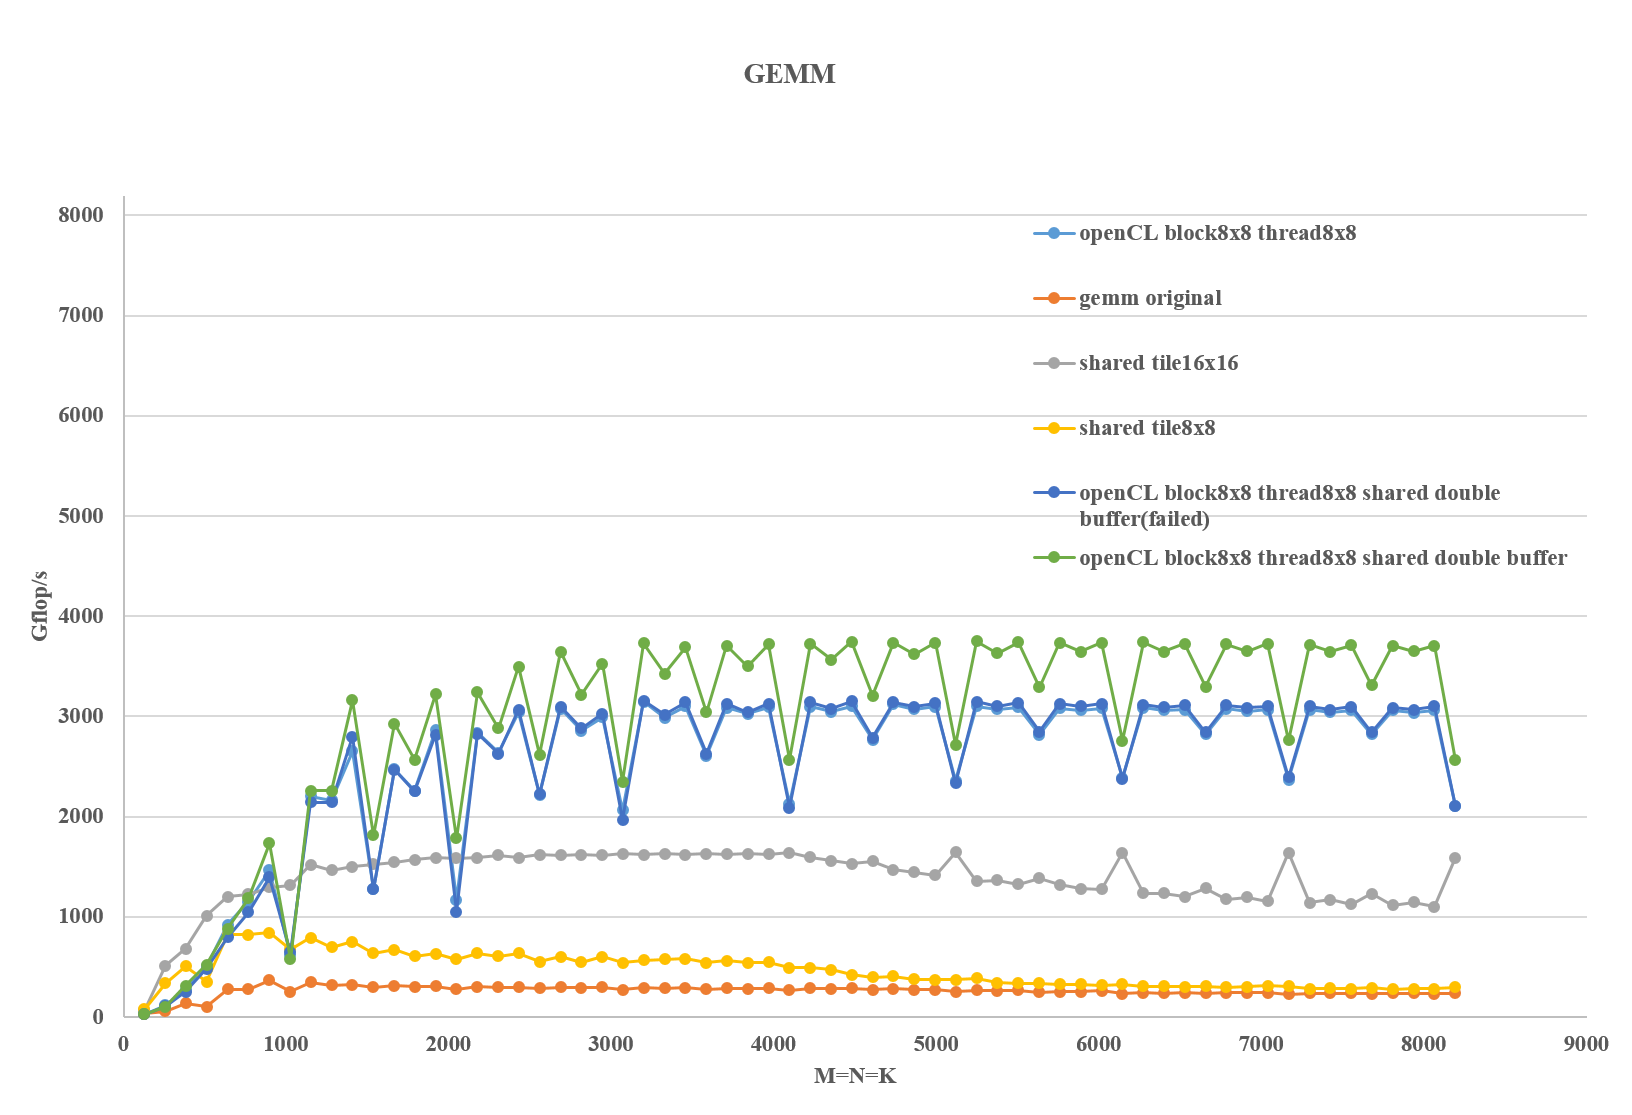
\includegraphics[width=0.80\textwidth]{opencl_gemm_1_1}
	\bicaption{矩阵乘OpenCL实现性能比较}{Comparison of GEMM performance implemented by OpenCL}
	\label{fig:opencl_gemm_1_1}
\end{figure}

从图\ref{fig:opencl_gemm_1_1}可以看出,最简单的矩阵乘GPU实现其浮点效率最低(图中橙色的gemm original)。gemm original实现没有使用shared memory,采用內积法每个线程计算一个输出。中间两条曲线表示使用shared memory,分块大小分别为8x8和16x16。由于矩阵乘在计算过程中有很多数据重用,利用数据重用的特点,将要计算的数据预先读入shared memory。在真正计算时从shared memory中取数据,可以减小数据读延迟。图\ref{fig:gemm_inner_product_tile}展示了使用shared memory分块的內积法矩阵乘。可以看出,计算C矩阵分块的同一行时,需要重复读A矩阵分块的同一行4个元素;同理,计算C矩阵分块的同一列时,要重复读B矩阵分块的同一列4个元素。全局内存读的次数减少4倍。分块大小为8时,全局内存读次数将减少8倍。所以在内存带宽受限时,提高shared memory分块大小可以减少全局内存读,降低内存带宽压力,提高计算性能。从图\ref{fig:opencl_gemm_1_1}中可以看出16x16分块的性能高于8x8分块。

\begin{figure}[htbp]
	\centering
	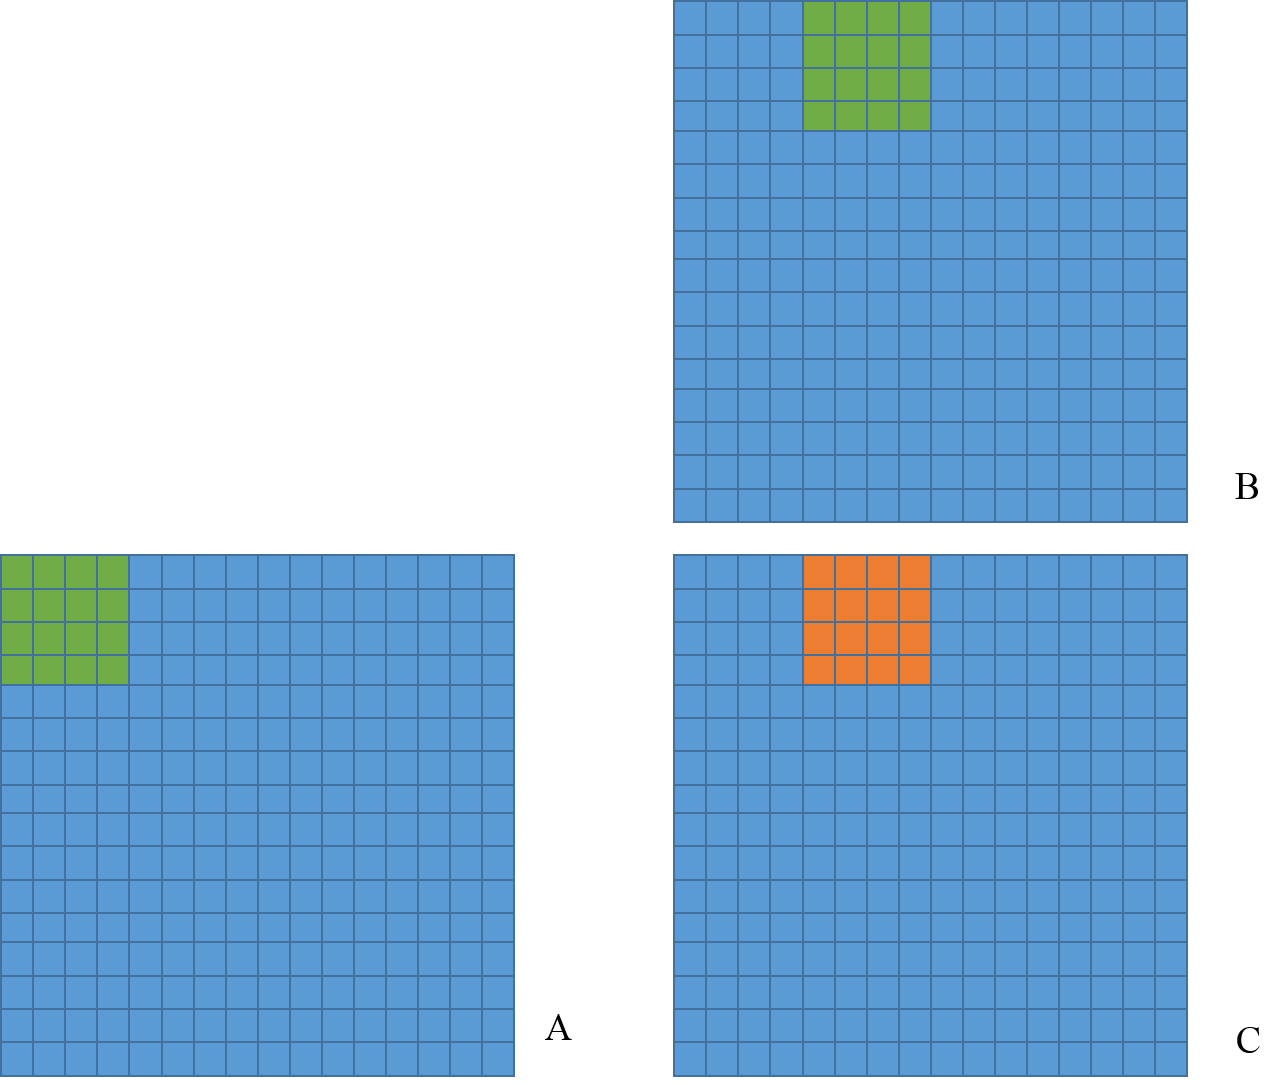
\includegraphics[width=0.60\textwidth]{gemm_inner_product_tile}
	\bicaption{內积法矩阵乘shared memory分块图示说明}{Illustration of inner-product GEMM with shared memory block}
	\label{fig:gemm_inner_product_tile}
\end{figure}

外积法矩阵乘的shared memory bank冲突分析:

图\ref{fig:shared_memory_bank_dist}展示了shared memory bank的分布情况。这里首先介绍一下AMD GPU shared memory的bank设计,shared memory有32的bank,每个bank的宽度为4字节。图\ref{fig:shared_memory_bank_dist}中绿色部分表示bank编号,蓝色部分表示一个block中A矩阵在shared memory中的分布情况,蓝色部分的同一列位于相同的bank。图中用其他颜色标注的部分,表示每个线程要读取的数据,例如(0,xxx)表示tid.x == 0 tid.y为0~7的线程要读取的8个元素。可以看出(0,xxx)线程和(4,xxx)线程都要读取bank0$\sim$bank7中的元素。图\ref{fig:bank0}展示了所有线程读bank0的情况。可以看出bank0的读取有4-way bank冲突。其他bank可类似分析。可以得知对于所有的bank,此时的shared memory有4-way bank冲突。

%bank冲突消除:


\begin{figure}[htbp]
	\centering
	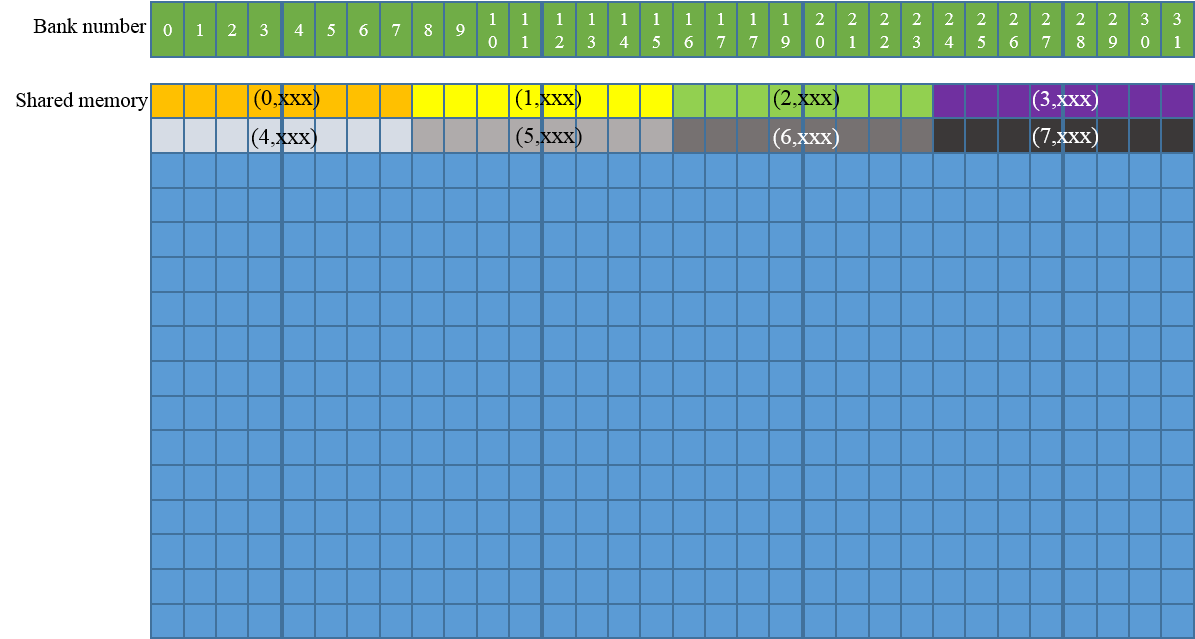
\includegraphics[width=0.80\textwidth]{shared_memory_bank_dist}
	\bicaption{shared memory bank分布}{Distribution of shared memory bank}
	\label{fig:shared_memory_bank_dist}
\end{figure}

\begin{figure}[htbp]
	\centering
	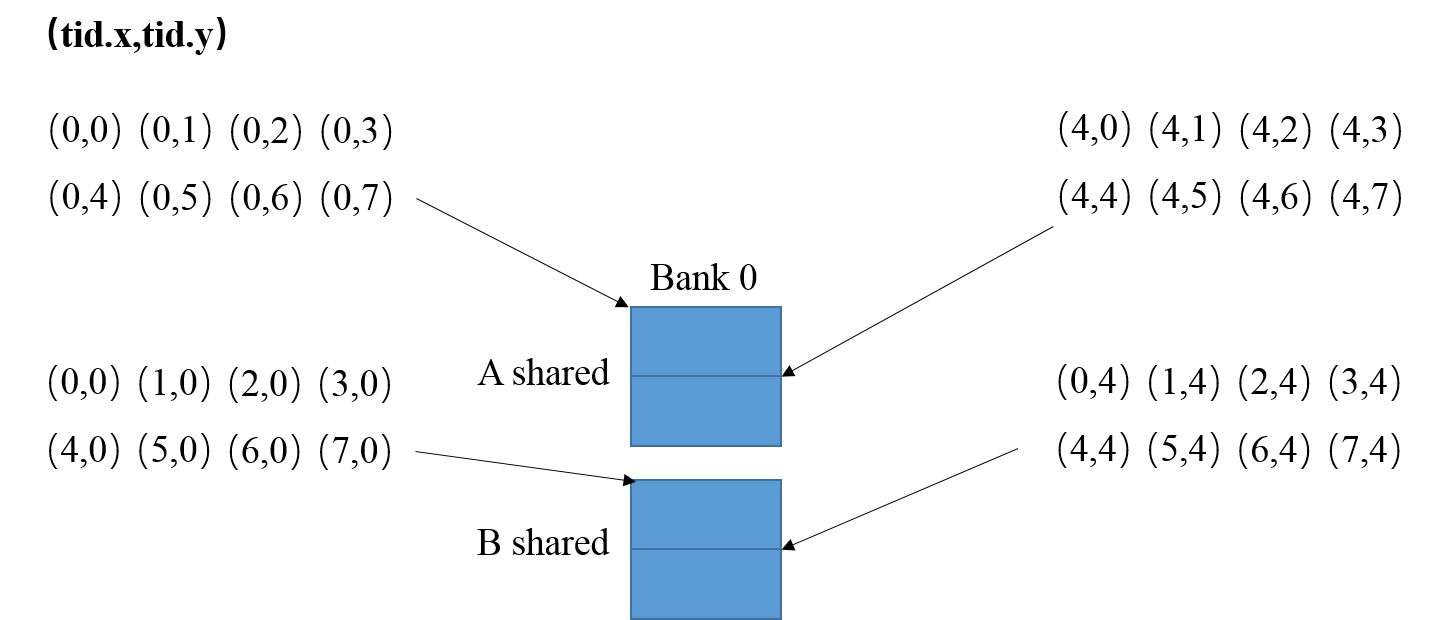
\includegraphics[width=0.80\textwidth]{bank0}
	\bicaption{4-way shared memory bank冲突}{4-way shared memory bank conflict}
	\label{fig:bank0}
\end{figure}

\subsection{优化内存访问}
汇编语言的访存优化和用高级语言(如CUDA,OpenCL)优化访存比较类似。一个wavefront(warp)中线程的全局访存请求可以合并成一到多个内存事务(memory transactions)。合并的方式和具体的GPU访存模式有关。为了高效的访问全局内存,通常我们安排一个wavefront中的线程访问全局内存中一段连续内存区域的数据。这样容易进行全局访存合并。在SGEMM程序的主循环中,主要的指令为v\_mac和ds\_read,为了提高v\_mac指令的百分比,减少ds\_read指令的数目就变得尤为关键。前面的介绍中,我们讲过可以通过使用DS\_READ\_B64或DS\_READ\_B128来减少DS\_READ指令数量。在shared memory中,线程读取A,B子矩阵也应该可以进行访存合并,我们安排每个线程可以读取连续的A,B子矩阵,一个wavefront中的线程可合并访问shared memory。同时,为了减少甚至消除shared memory的bank冲突和满足DS\_READ指令对齐的要求,在必要的时候,我们需要在shared memory中合理的进行填充。


\subsection{循环展开}
通过循环展开(如图\ref{fig:loop_unroll}),我们可以提高指令的通量。如下图中所示,我们沿着K方向做循环展开,这样在每次循环产生更多的浮点乘加操作,充分利用GPU上每个线程可拥有的寄存器个数。并且以循环展开作为前提,我们可以做后续的寄存器双缓冲,局部共享内存双缓冲等优化。通常我们都是做偶数次展开,这是为后面双缓冲要恰好是2的倍数做准备在这里,我们循环展开8次,这里考虑的因素有寄存器个数的限制,和局部共享内存的限制。

\begin{figure}[htbp]
	\centering
	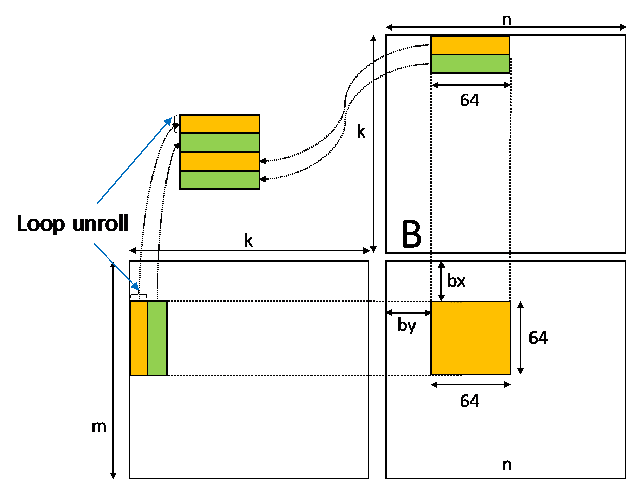
\includegraphics[width=0.50\textwidth]{loop_unroll}
	\bicaption{循环展开图示}{Loop unroll}
	\label{fig:loop_unroll}
\end{figure}

\subsection{数据预取}
为了减小计算时,读取数据产生的等待延迟,我们进行数据的预取。

从全局内存预取数据到共享内存,我们以增加一倍局部共享内存的代价来掩盖全局内存的访存延迟;从局部共享内存预取数据到寄存器,我们以增加一倍寄存器的代价来掩盖局部共享内存访存的延迟。

\subsection{shared memory双缓冲}
在前面的矩阵乘GPU算法描述中,讲述了shared memory的使用方法。首先将数据从全局内存读入寄存器,然后从寄存器写回到shared memory,最后再从shared memory读取数据到寄存器,并在寄存器中做计算。

为了更有效地利用shared memory,我们采用shared memory双缓冲。如算法\ref{alg:gemm_sharedmem}所示,首先从全局内存预取数据到寄存器,然后从寄存器写回到shared memory。在从shared memory读取数据到寄存器并做计算之前,从全局内存预取下一次要计算的数据到寄存器。在OpenCL的实现中,shared memory双缓冲带来了$\sim$7.8\%的性能提升(如图\ref{fig:gemm_shared_double_buffer})。
\begin{figure}[htbp]
	\centering
	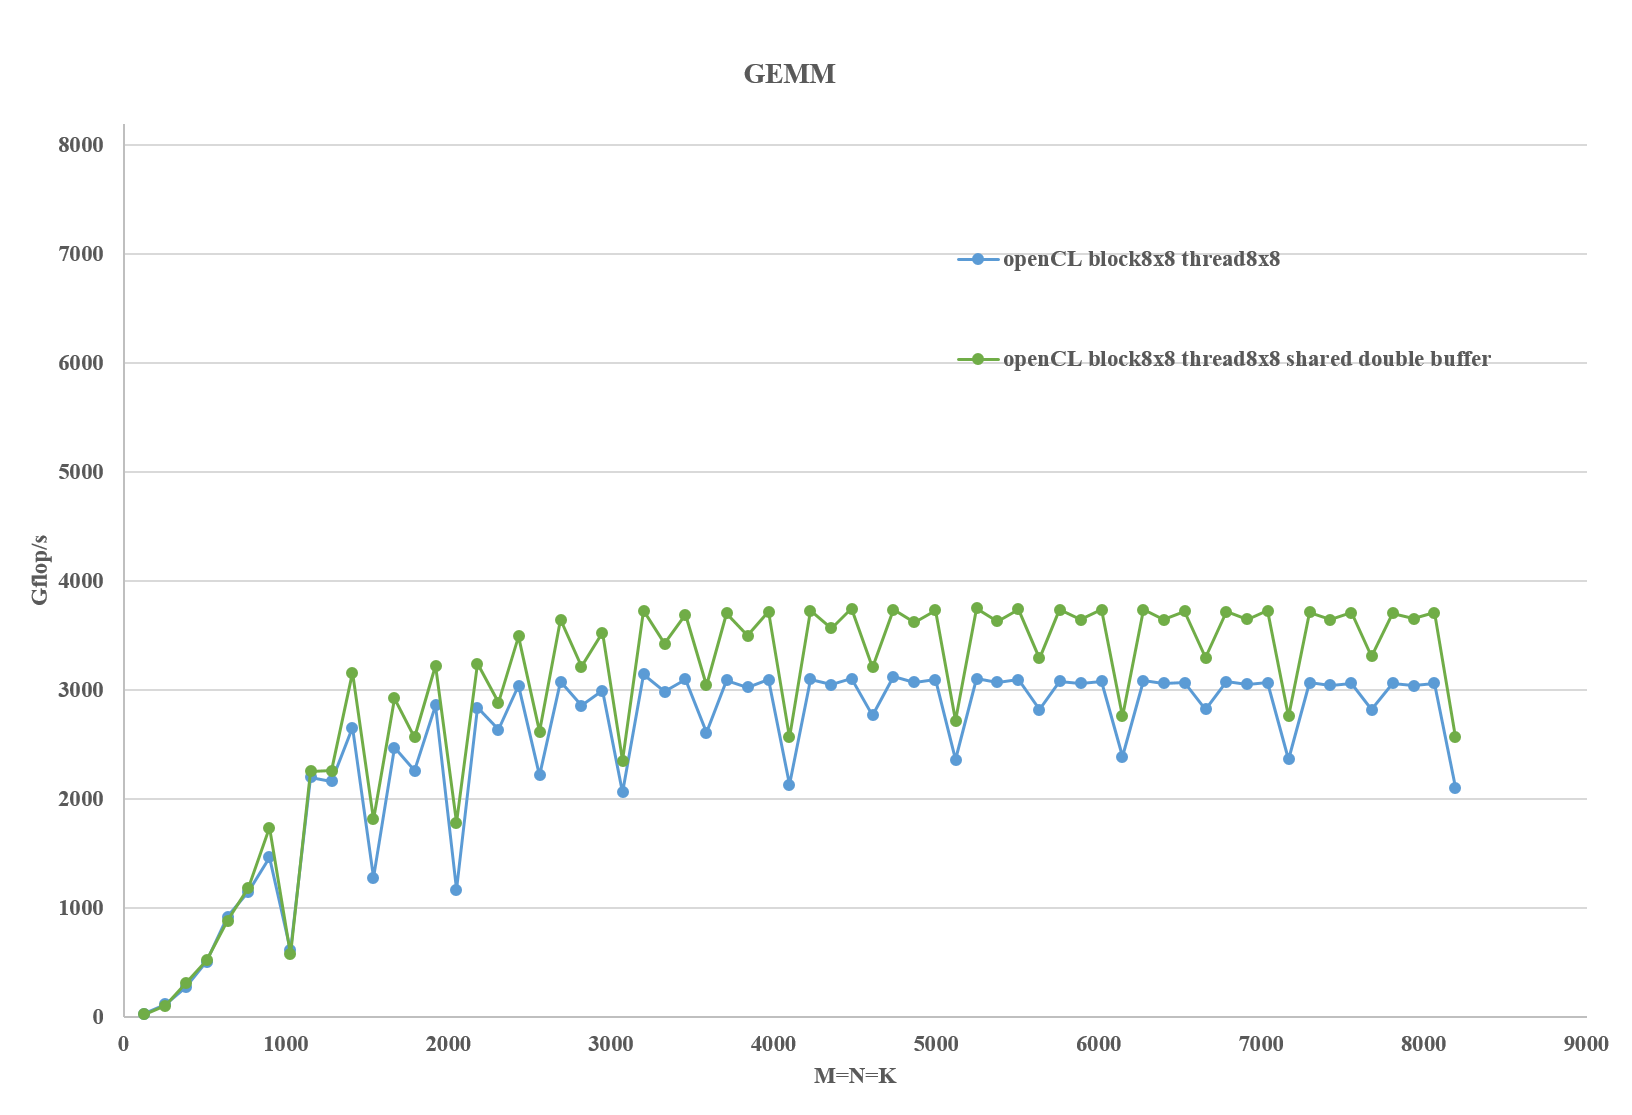
\includegraphics[width=0.80\textwidth]{gemm_shared_double_buffer}
	\bicaption{shared memory双缓冲带来的性能提升}{Shared memory double buffering brings performance improvements}
	\label{fig:gemm_shared_double_buffer}
\end{figure}

\begin{algorithm}[htbp]
	\small
	\caption{GEMM algorithm with shared memory double buffer}\label{alg:gemm_sharedmem}
	\begin{algorithmic}[1]
		%\Procedure{Euclid}{$a,b$}\Comment{The g.c.d. of a and b}
		\State $A, B, C$\Comment{matrix A, B, C}
		\State $regA[task\_size],regB[task\_size],regC[task\_size]$\Comment{Allocate register for compute}
		\State $tileA[tile\_length*NUM\_UNROLL],tileB[tile\_length*NUM\_UNROLL]$\Comment{Shared memory double buffer}
		\State $tileA'[tile\_length*NUM\_UNROLL],tileB'[tile\_length*NUM\_UNROLL]$
		\State $loadA[tile\_length*NUM\_UNROLL/threadblock]$\Comment{Register for global memory load}
		\State $loadB[tile\_length*NUM\_UNROLL/threadblock]$
		\State $regC \gets 0$
		\State $loadA \gets A, loadB \gets B $\Comment{Pre load tile of A, B from global to register}
		\State barrier CLK\_GLOBAL\_MEM\_FENCE
		\For   {$i = 0$; $i < K/NUM\_UNROLL$; $++i$}
			\If    {$i \% 2 == 0$}
				\State $tileA \gets loadA, tileB \gets loadB$
				\State barrier CLK\_LOCAL\_MEM\_FENCE
				\State $loadA \gets A, loadB \gets B $\Comment{Load the next tile of A, B from global to register}
				\State barrier CLK\_GLOBAL\_MEM\_FENCE
					\For   {$k = 0$; $k<NUM\_UNROLL$;$++k$}\Comment{Loop Unroll}
						\State $regA \gets tileA, regB \gets tileB$
						\State $regC += regA \cdot regB$
					\EndFor
			\Else  
				\State $tileA' \gets loadA, tileB' \gets loadB$
				\State barrier CLK\_LOCAL\_MEM\_FENCE
				\State $loadA \gets A, loadB \gets B $\Comment{Load the next tile of A, B from global to register}
				\State barrier CLK\_GLOBAL\_MEM\_FENCE
					\For   {$k = 0$; $k<NUM\_UNROLL$;$++k$}\Comment{Loop Unroll}
						\State $regA \gets tileA', regB \gets tileB'$
						\State $regC += regA \cdot regB$
					\EndFor
			\EndIf
			\State barrier CLK\_LOCAL\_MEM\_FENCE
		\EndFor\label{gemmendfor}
		\State $C \gets regC$\Comment{Store C from registers to global memory}
		%\EndProcedure
	\end{algorithmic}
\end{algorithm}

\subsection{寄存器双缓冲}
如图\ref{fig:reg_double_buffer}所示,我们可以在用寄存器A1,B1计算的同时,从局部共享内存取下一次要计算的数据到寄存器A0,B0。由于数据的预取,在进入循环前,我们已经将第一次要计算的数据读到了寄存器A0[0:7],B0[0:7] 中。

每个线程使用A1,B1寄存器中的数据,做本次的8x8乘加操作;在线程做本次乘加操作的同时,从局部共享内存预取下一次的数据到寄存器A0,B0。通过寄存器双缓冲,我们可以用计算掩盖从局部共享内存读的延迟。我们沿着K方向循环展开8次,分成0,2,4,6 和 1,3,5,7 一半奇数,一半偶数。偶数次时,每个线程从shared memory预取8个a到寄存器A1[0:7],8个b到寄存器B1[0:7], 即预取下一次(奇数时)计算需要的8个a和8个b。奇数次时,每个线程从shared memory预取8个a到寄存器A0[0:7],8个b到寄存器B0[0:7], 即预取下一次(偶数时)计算需要的8个a和8个b。偶数次循环计算A0[0:7]*B0[0:7],奇数次循环计算 A1[0:7]*B1[0:7]。对每个线程来说,需要计算8x8个输出,共需要做64次乘加操作。从共享内存读,一次读4个连续元素,读8个a和8个b,需要4个共享内存读指令。这样,我们就可以用寄存器的计算,来掩盖共享内存读的延迟。

\begin{figure}[htbp]
	\centering
	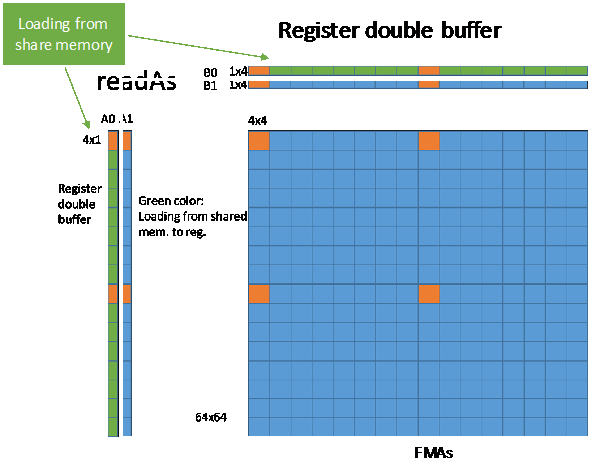
\includegraphics[width=0.50\textwidth]{reg_double_buffer}
	\bicaption{寄存器双缓冲}{Register double buffer}
	\label{fig:reg_double_buffer}
\end{figure}

\subsection{线程负载均衡}
对每个线程来说,我们使用4个4x4,来代替8x8的计算方式,来使得一个block中的线程可以负载均衡(如图\ref{fig:load_balance})。通过这种方式,我们可以提高一个block的计算效率。
\begin{figure}[htbp]
	\centering
	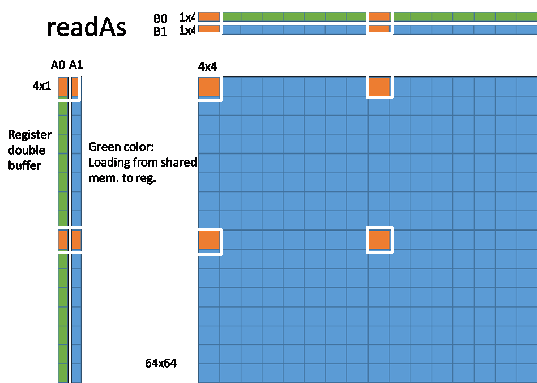
\includegraphics[width=0.50\textwidth]{load_balance}
	\bicaption{线程负载均衡}{Thread load balance}
	\label{fig:load_balance}
\end{figure}


\subsection{消除shared memory bank冲突}
AMD GPU shared memory有32个bank。当不同的线程访问不同的bank时,线程可以同时读;当不同的线程访问同一个bank的同一个位置时,可以进行广播;当不同的线程访问同一个bank的不同位置时,会产生bank冲突,需要多个时钟周期来完成。所以,bank冲突会减小访存带宽,对性能影响很大。

下图中小方格中的数字表示一个block中的64个线程,我们将64个线程看成一个2维的线程数组tid.x 取值从0~7, tid.y取值从0~7

小方格中的数字对(tid.x,tid.y)对应的线程号为tid = tid.y * 8 + tid.x

我们可以看到,图\ref{fig:bank_conflict}中同一行的线程读4个连续的bank,没有bank冲突;不同线程读相同的位置,会在同一行进行广播;图中同一列的线程读4个连续的bank,没有bank冲突,会在同一列进行广播。因此,通过设计这种共享内存读的方式,我们可以完全消除bank冲突。
\begin{figure}[htbp]
	\centering
	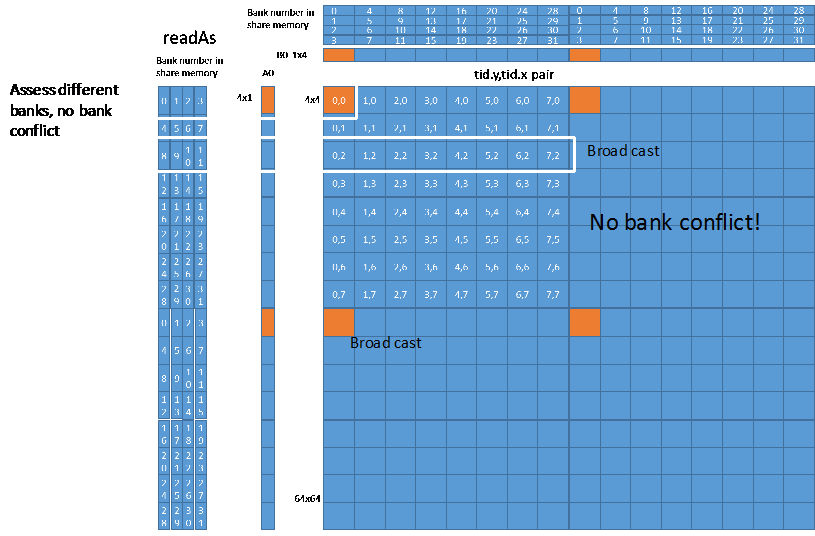
\includegraphics[width=0.50\textwidth]{bank_conflict}
	\bicaption{shared memory bank冲突消除}{Shared memory bank conflict elimination}
	\label{fig:bank_conflict}
\end{figure}


\subsection{指令重排}
通常,我们尝试将不同类型的指令交错放置来使得一个CU上不同的功能部件可以均衡的利用起来,进而获得更高的指令通量。我们采用下面的指令重排方法:

将全局内存数据预取指令和v\_mac,DS\_READ指令交错放置来获得更高的性能。

\subsubsection{指令重排的几个原则}
(1) 从shared memory中预取数据到寄存器的指令:尽可能地早放置

ds\_read\_b128指令:从shared memory中预取数据到寄存器。

循环展开8次,每次计算8x8个输出。总共8x8x8 = 512条v\_mac指令。一条ds\_read\_b128指令可以从shared memory中取4个浮点元素。计算8x8的输出需要8个A中对应元素和8个B中对应元素,因此需要(8+8)/4 = 4 条ds\_read\_b128指令。在计算本次8x8个v\_mac时,要预取下一个8x8个v\_mac所需的指令。为了给ds\_read\_b128指令从发射到结果返回留出足够多的时间,我们放置ds\_read\_b128指令的原则是尽可能地早发射ds\_read\_b128指令,所以我们在每次8x8个v\_mac最开始的位置之前插入4条ds\_read\_b128指令。

(2) 从全局内存读取数据到寄存器:尽可能地早放置

t\_buffer\_load\_xyzw指令:从全局内存预取数据到寄存器。

一个block有64个线程,每个线程计算8x8个输出,总共可以计算64x64个输出。t\_buffer\_load\_xyzw指令一次可以从全局内存读取4个元素,计算64x64的输出,循环展开8次,需要8x64个A中对应元素和8x64个B中对应元素。因此每个线程需要(8x64+8x64)/(4x64) = 4条t\_buffer\_load\_xyzw指令。

(3) 从寄存器写入数据到shared memory:和全局内存读指令间隔足够远

为了数据重用,我们把从全局内存读到寄存的数据写入shared memory。使用ds\_read\_b128指令将数据从存寄存器写入shared memory。ds\_read\_b128指令要等对应的t\_buffer\_load\_xyzw指令结果返回,所以ds\_read\_b128指令和t\_buffer\_load\_xyzw要间隔得足够远。

\section{矩阵乘性能测试}
\begin{figure}[htbp]
	\centering
	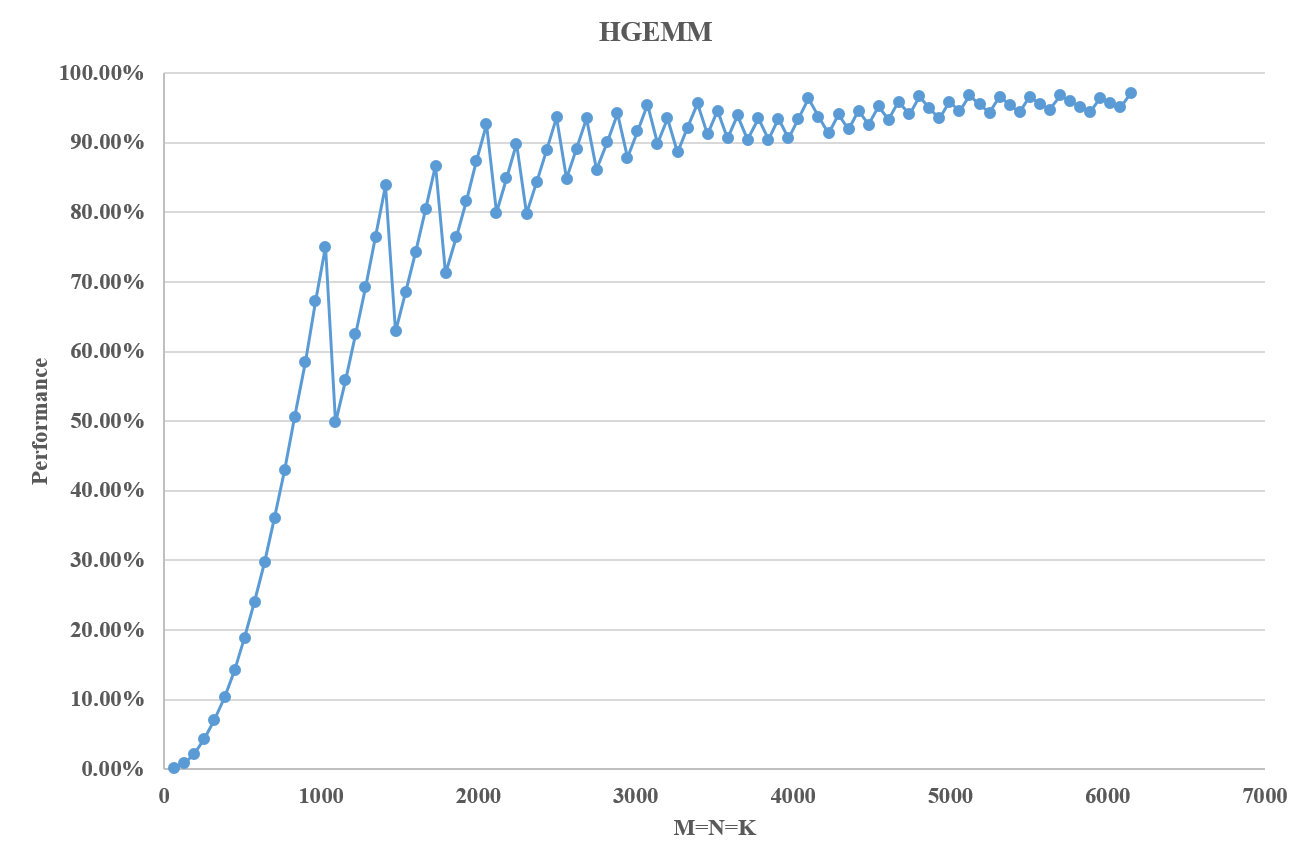
\includegraphics[width=0.80\textwidth]{hgemm_perf}
	\bicaption{矩阵乘性能变化趋势}{GEMM performance}
	\label{fig:hgemm_perf}
\end{figure}

通过实际测试,我们的矩阵乘性能峰值可达95\%。

\section{矩阵乘性能分析}
\subsection{矩阵乘潜在性能峰值}
在寄存器分块大小为8x8,block线程数为64的情况下。v\_mac峰值性能为512/(512+24+2)= 512/538 = 95.17\%。这里在计算上认为32条ds\_read\_b128有只有8条指令双发射。实际处理器的执行行为需要通过测试可以得知。如果在执行时,将每4条ds\_read\_b128指令合并,则32条ds\_read\_b128全部都双发射。此时的v\_mac峰值性能为512/(512+2)= 99.61\%(如图\ref{tab:fijiFFMA})。

\begin{table}[htbp]
	\bicaption{矩阵乘主循环指令构成}{GEMM main loop instructions}
	\label{tab:fijiFFMA}
	\begin{center}
		\begin{tabular}{ | l | p{4cm} |}
			\hline
			Operation & Count \\ \hline
			v\_mac & 512  \\ \hline
			ds\_read\_b128 & total 32, 8 dual issue \\ \hline
			ds\_write\_b128 & 4 dual issue \\ \hline
			tbuffer\_load\_xyzw & 4 dual issue \\ \hline
			v\_add\_u32 & 2 \\ \hline
			s\_waitcnt vmcnt() & 4 dual issue \\ \hline
			s\_add\_u32 & 1 dual issue \\ \hline
			s\_cmp\_gt\_u32 & 1 dual issue \\ \hline
			s\_cbranch\_scc0 & 1 daul issue \\
			\hline
		\end{tabular}
	\end{center}	
\end{table}

%\subsection{Roofline模型}

\section{本章小结}
本章首先介绍了本次实验所使用的计算环境。然后讲述了寄存器分块的大小和读数据指令的位宽对浮点通量的影响。接下来,详细描述了矩阵乘汇编调优的过程,最后进行了矩阵乘性能上界分析。


